\chapter{Ergebnisse und Diskussion}

\begin{figure}[position=h]
  \centering
  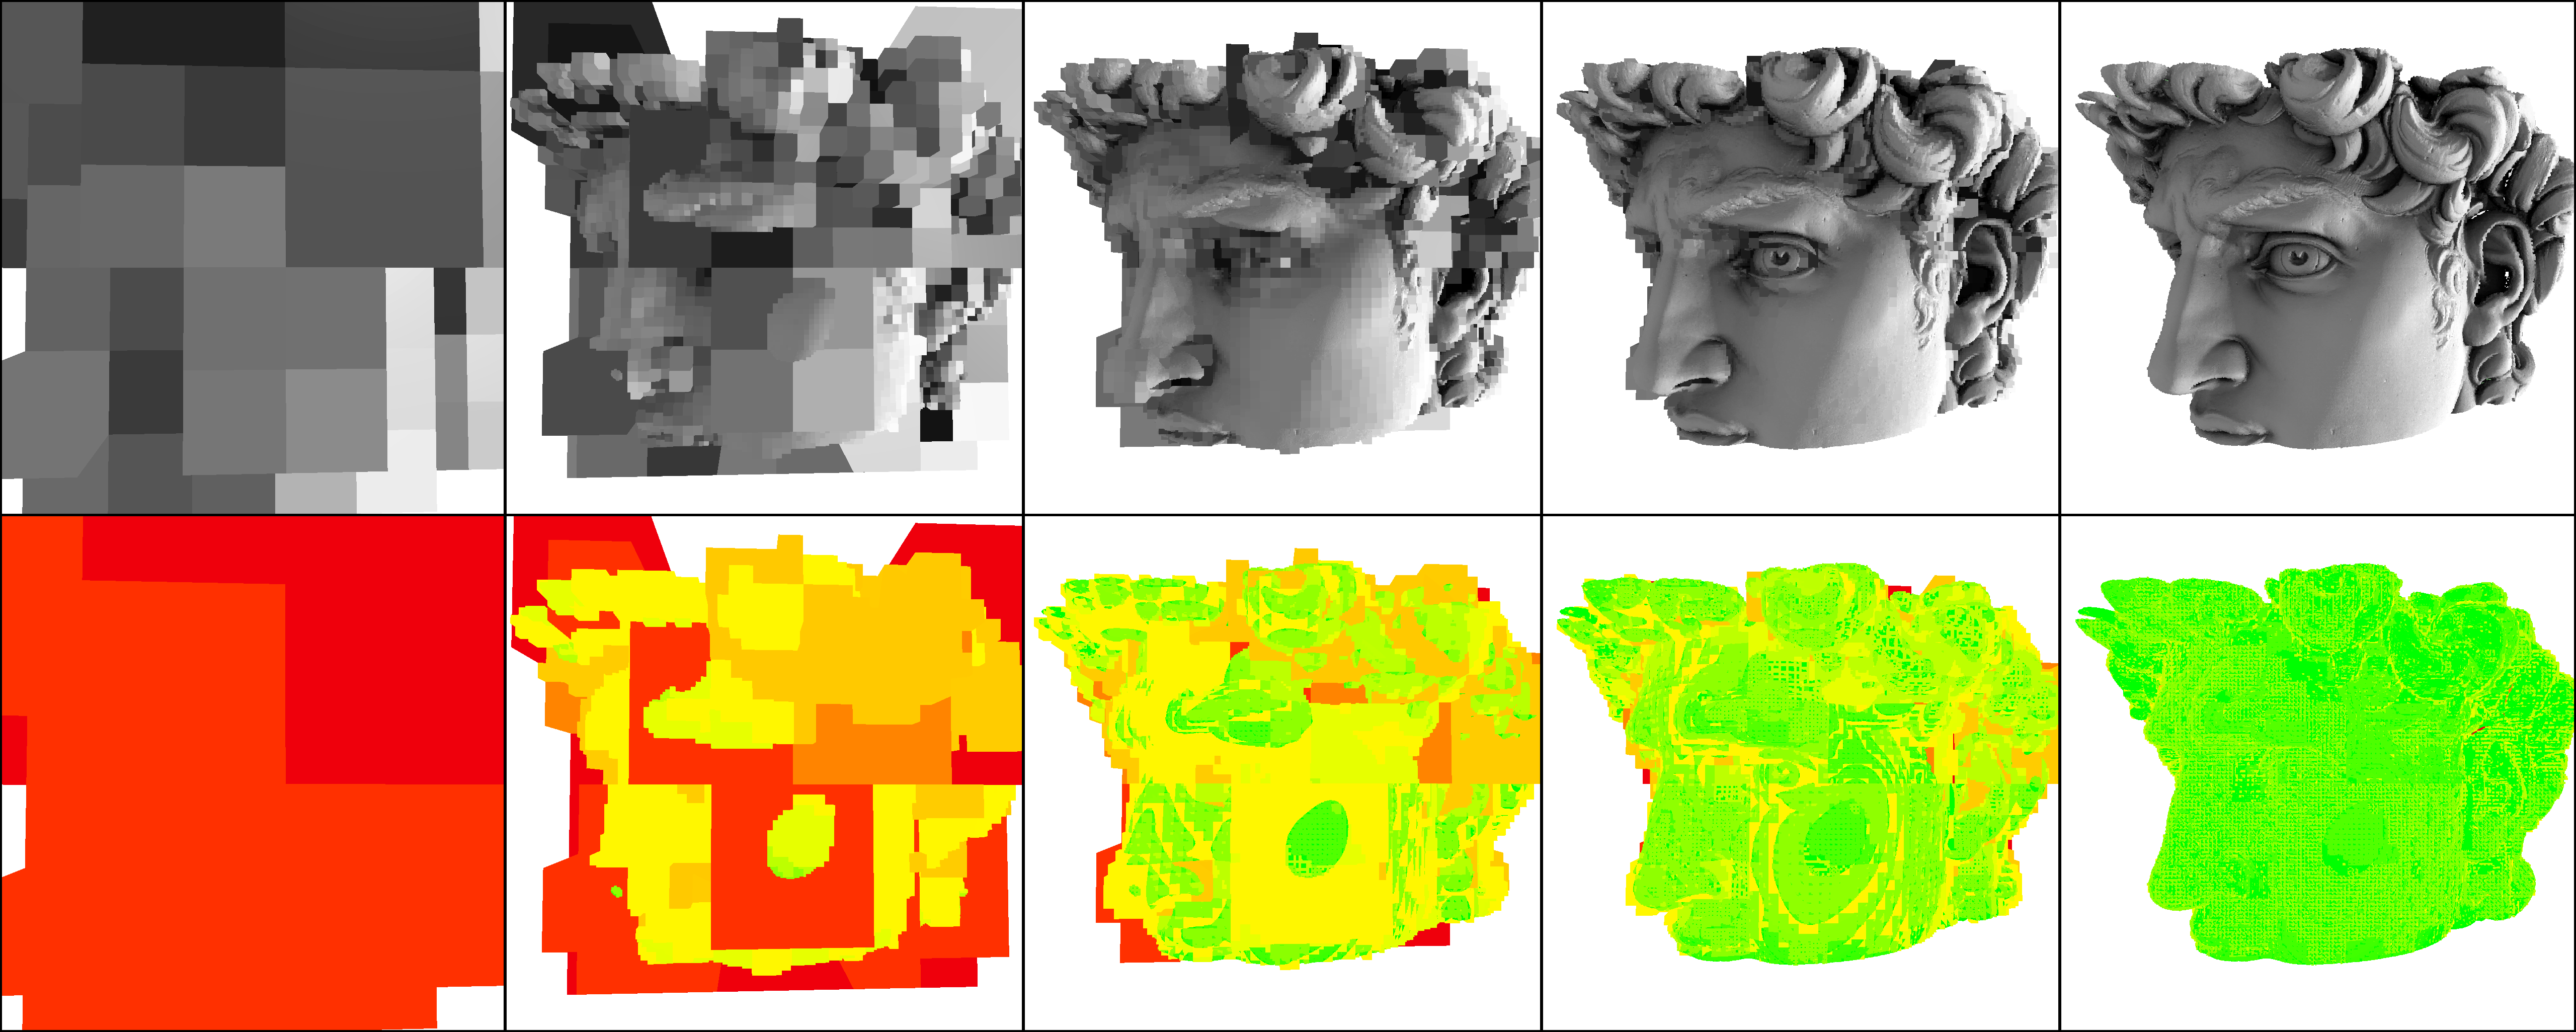
\includegraphics[width=1.0\textwidth]{figures/progressive_refinement.png}
  \caption{Verfeinerung in 5 aufeinander folgenden Schritten \label{progressive_refinement}}
\end{figure}

\section{�berblick}
\section{Verwendete Testszenen}
 

Zum Testen des Out-of-Core Systems wurden SVO-Strukturen f�r drei unterschiedliche Geometrien generiert (siehe Tabelle ...). 
Aus jeder Geometrie wurden zwei verschiedene SVO-Strukturen erstellt. Beide haben jeweils die selbe minimale Tiefe, aber eine unterschiedliche Treelet Gr��e. Die Tiefe betrug jeweils 12 bei Treelet Gr��en von 1kb und 4kb. Durch die Verkleinerung der Treelets bei gleicher minimaler SVO-Tiefe entstehen mehr Treelets und damit eine gr��erer Aufwand bei der Verwaltung. Die beiden Varianten sollen im folgenden verglichen werden, um die Skalierbarkeit des Out-of-Core Systems nach zu vollziehen. In Tabelle ... wird gezeigt... .

\begin{table}
\centering
\begin{tabular}{ l  r  r }
  \hline
  \textbf{Name} & \textbf{Anzahl Dreiecke} & \textbf{Dateigr��e} \\
  \hline
  David face       & 52.5 Mio & 14.7 GB \\
  \hline
  xyzrgb statuette & 10.0 Mio & 270 MB \\
  \hline  
  Lucy             & 28.0 Mio & 757 MB  \\
  \hline
\end{tabular}

\caption{Verwendete Modelle}\label{verwendete_modelle}
\end{table}




\begin{table}
\centering
\begin{tabular}{ l  r  r  r  r  r }
  \hline
  \textbf{Name} &  & \textbf{Treelet Gr��e} & \textbf{Anzahl Treelets} & \textbf{Anzahl Knoten} & \textbf{Dateigr��e} \\
  \hline
  David face        & 1kb & 743.277 &  95.139.456  & 000000\\
                    & 4kb & 484.297 & 247.960.064  & 000000\\
  \hline
  xyzrgb statuette  & 1kb & 13      & 000000      & 000000 \\
                    & 4kb & 13      & 000000      & 000000 \\
  \hline  
  Lucy              & 1kb & 13      & 000000      & 000000 \\
                    & 4kb & 13      & 000000      & 000000 \\
  \hline
\end{tabular}

\caption{Verwendete Modelle}\label{verwendete_modelle}
\end{table}
 
 

\section{Laufzeitanalyse}
Zum Testen wurden die Zeiten f�r die einzelnen Verarbeitungsschritte des Out-of-Core Systems gemessen. W�hrend der Messung wurde die Bildsynthese deaktiviert, um ausschlie�lich den Einfluss der Anzahl der Treelets auf den Ver\-walt\-ungsaufwandes zu untersuchen. Der SVO wurde �ber einen Zeitraum von 60 Sekunden aus verschiedenen Perspektiven analysiert und verfeinert. Durch die kontinuierliche Ver�nderung der Perspektive muss das System permanent neue Teile des Octrees anfordern, w�hrend es andere verwerfen muss. Damit bei der Verfeinerung auch Treelets in hohen Octree Tiefen angefordert werden, wird zum testen eine Kamerafahrt verwendet die ein Ma� an Koh�renz zwischen den Perspektiven zu gew�hrleisten.

\begin{figure}[position=h]
  \centering
  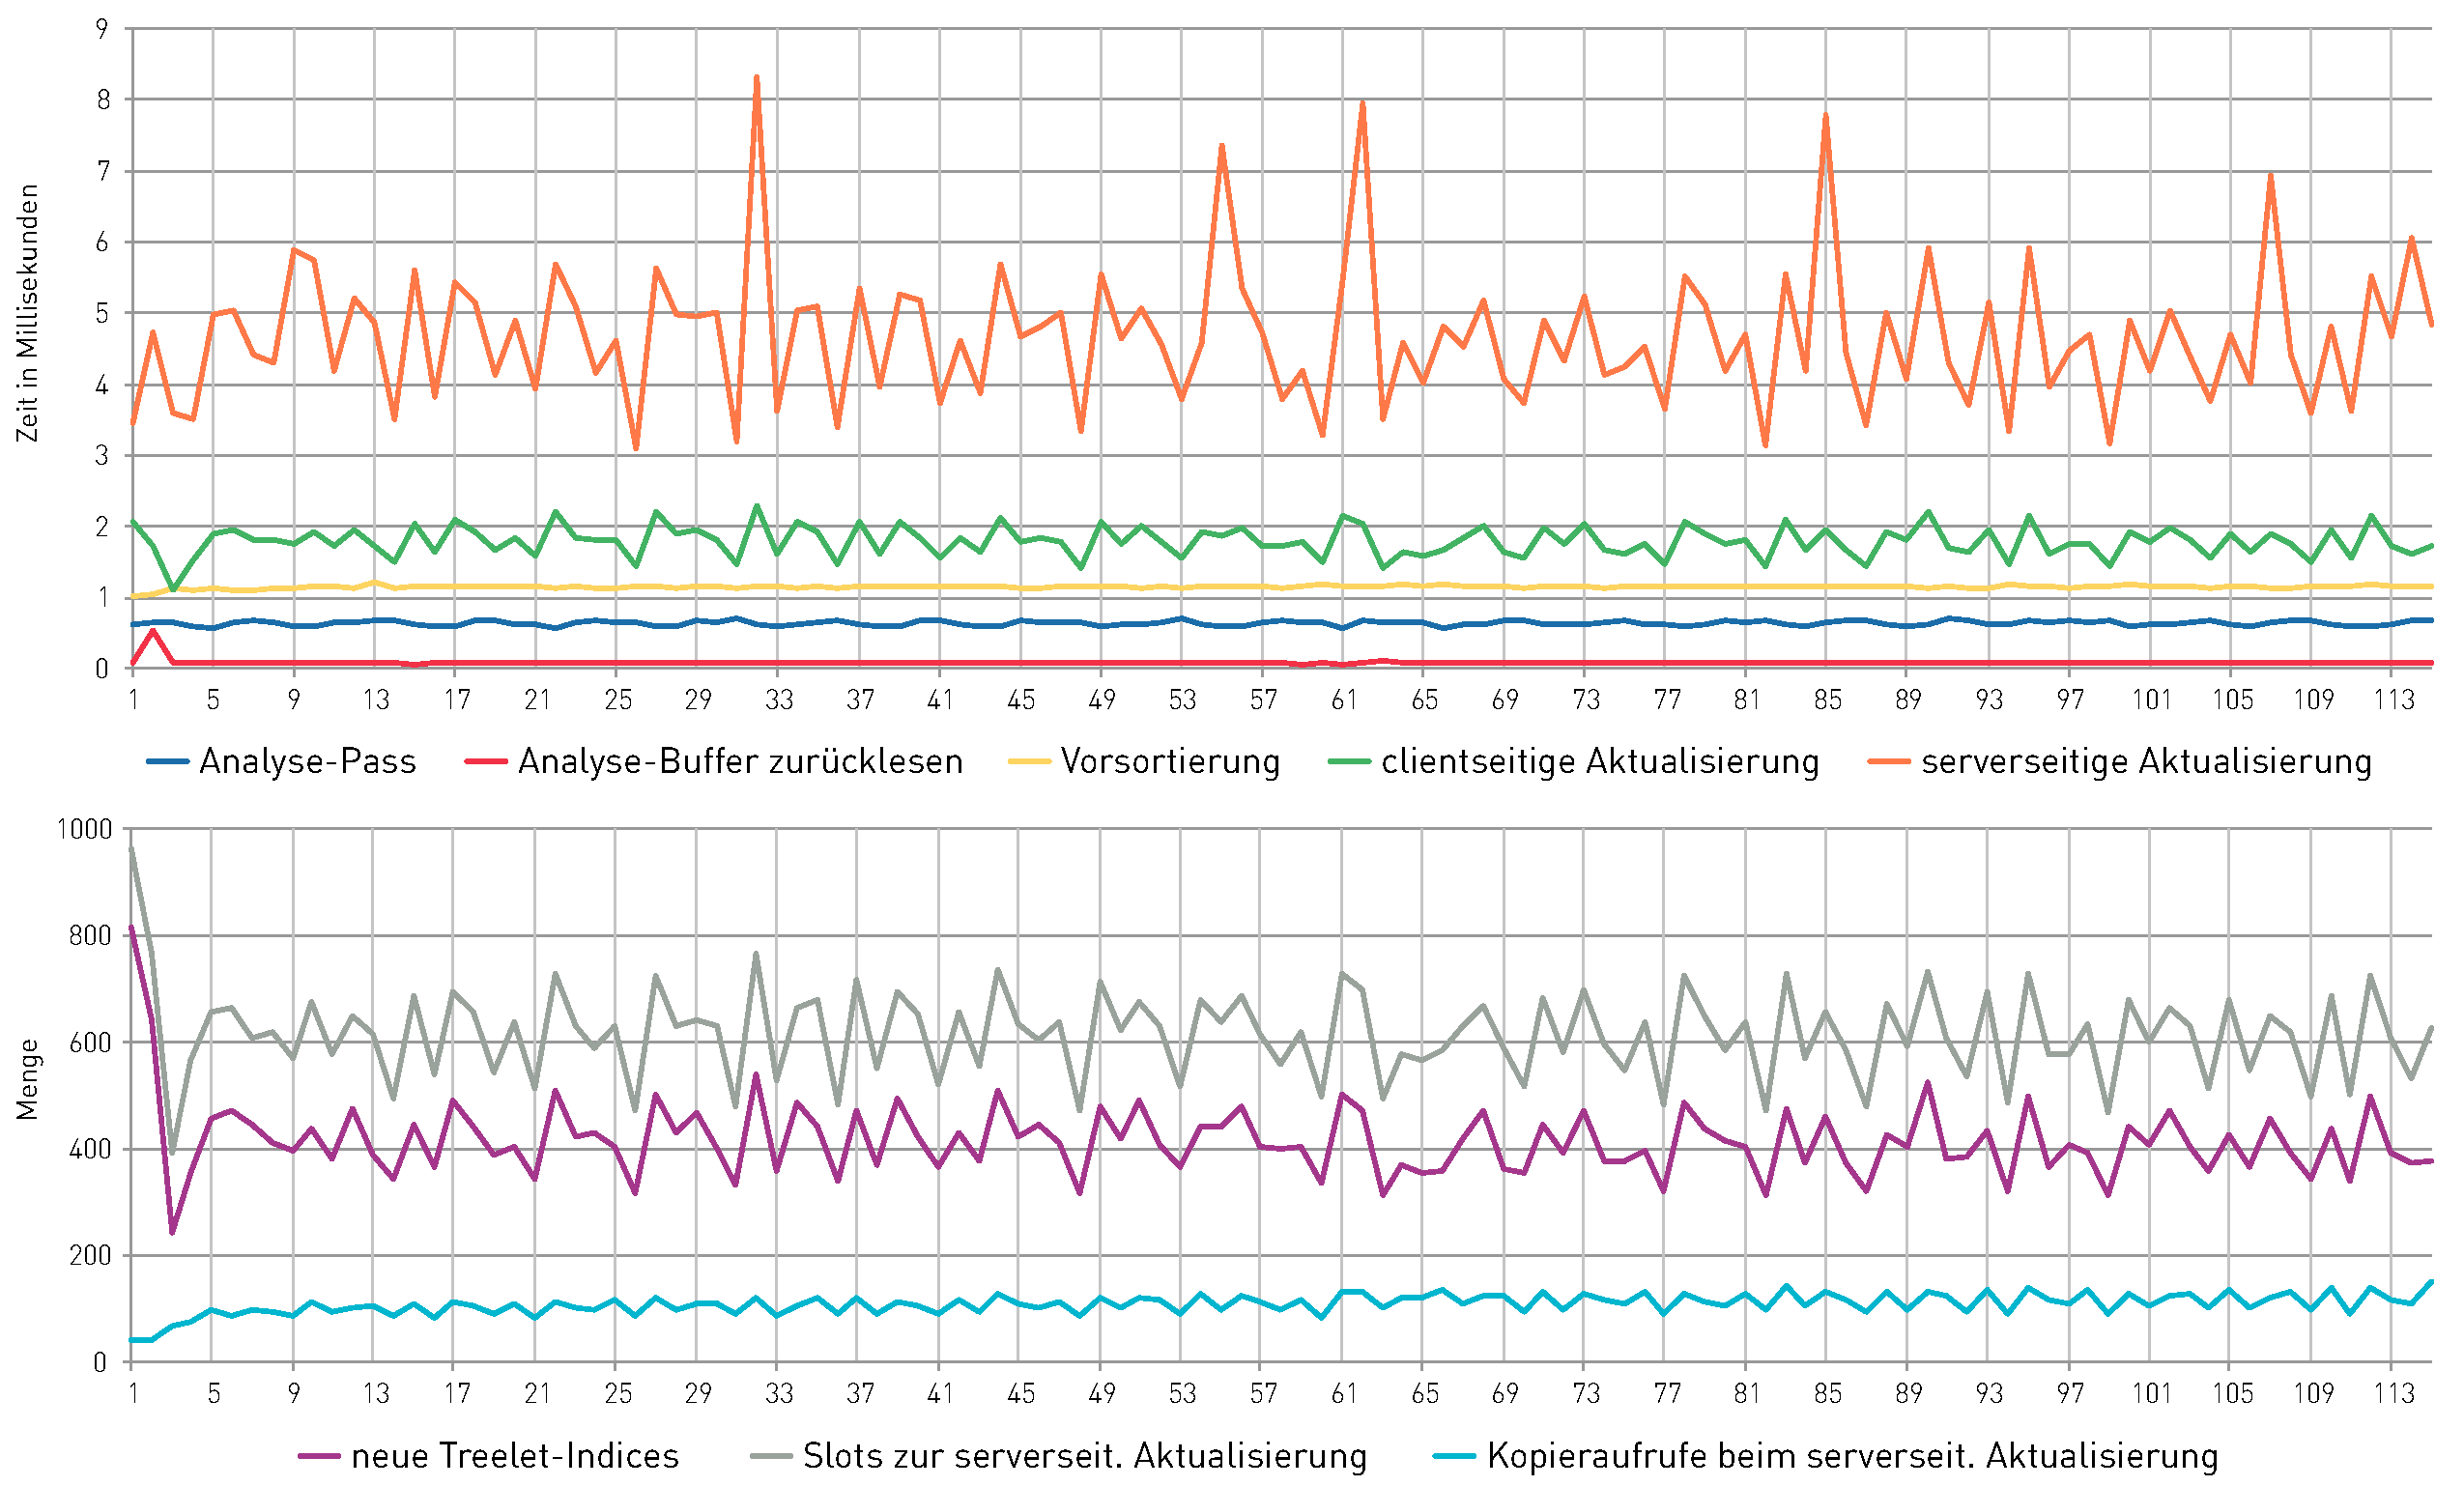
\includegraphics[width=1.0\textwidth]{figures/lucy_s4_D13_timeseries.pdf}
  \caption{Systemzeiten und Arbeit f�r Model lucy mit 4 kb Treelets\label{lucy_s4_D13_timeseries}}
\end{figure}

\begin{figure}[position=h]
  \centering
  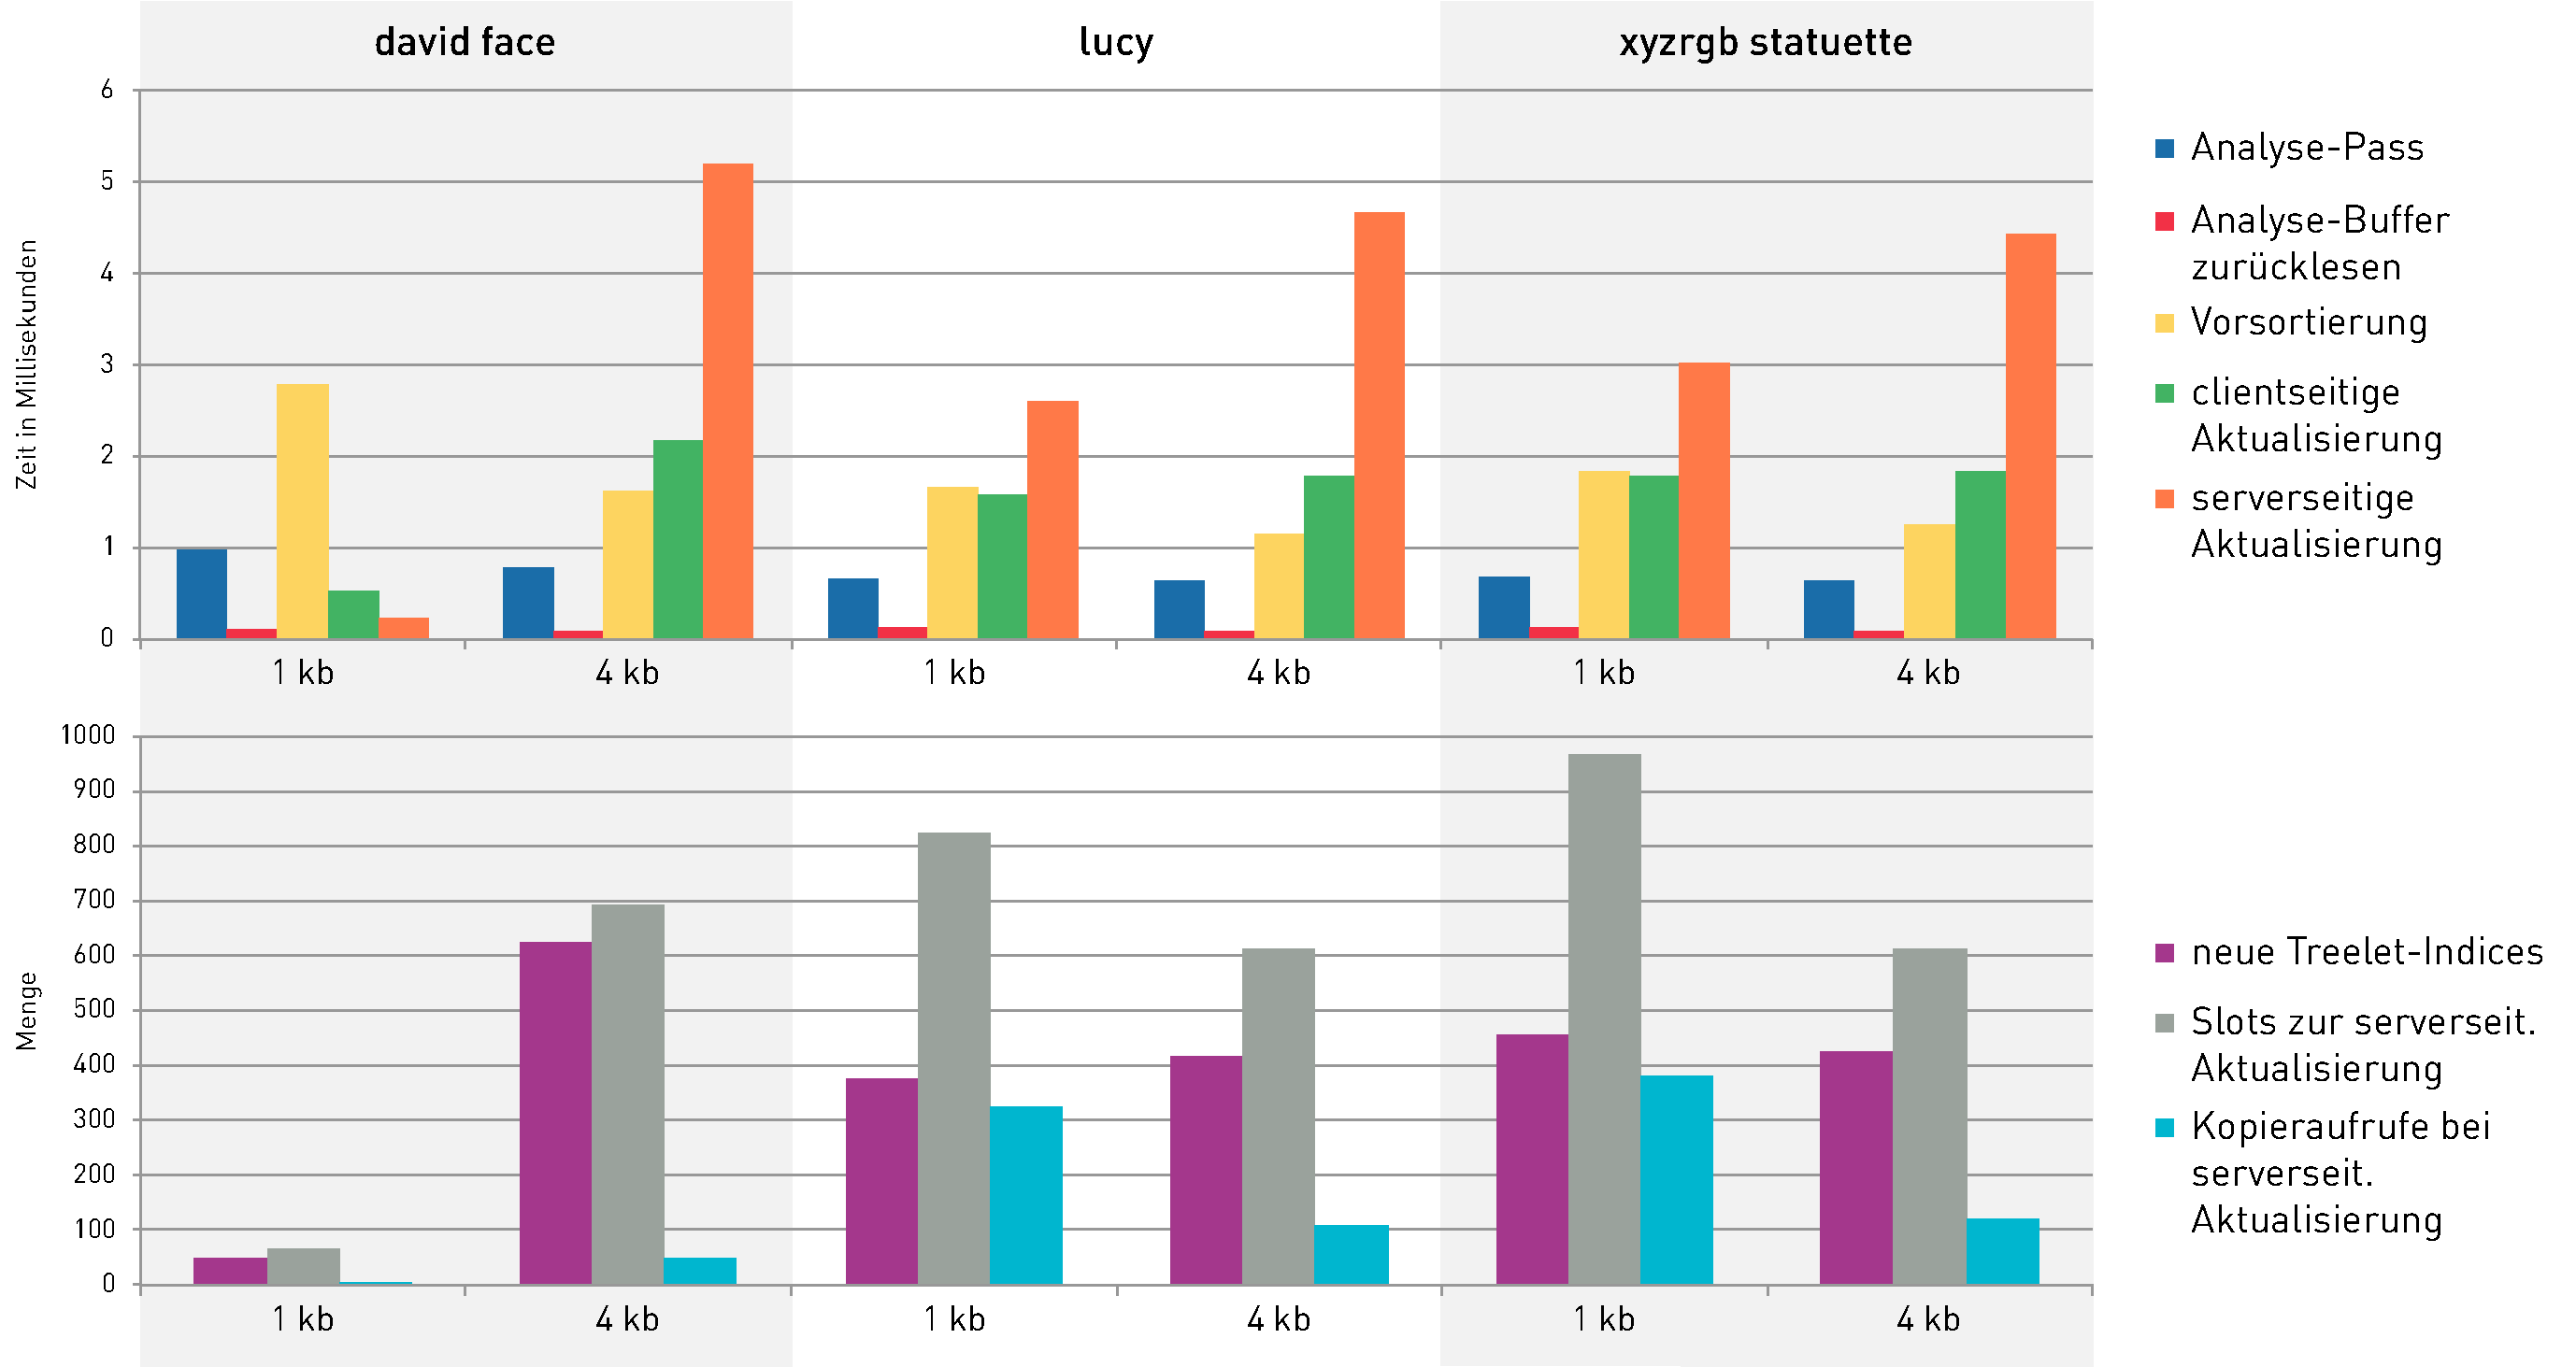
\includegraphics[width=1.0\textwidth]{figures/david_lucy_xyzrgb_s1_vs_24_D13.pdf}
  \caption{Gegen�berstellung unterschiedleichen Treelet-Gr��en\label{david_lucy_xyzrgb_s1_vs_24_D13}}
\end{figure}

\begin{figure}[position=h]
  \centering
  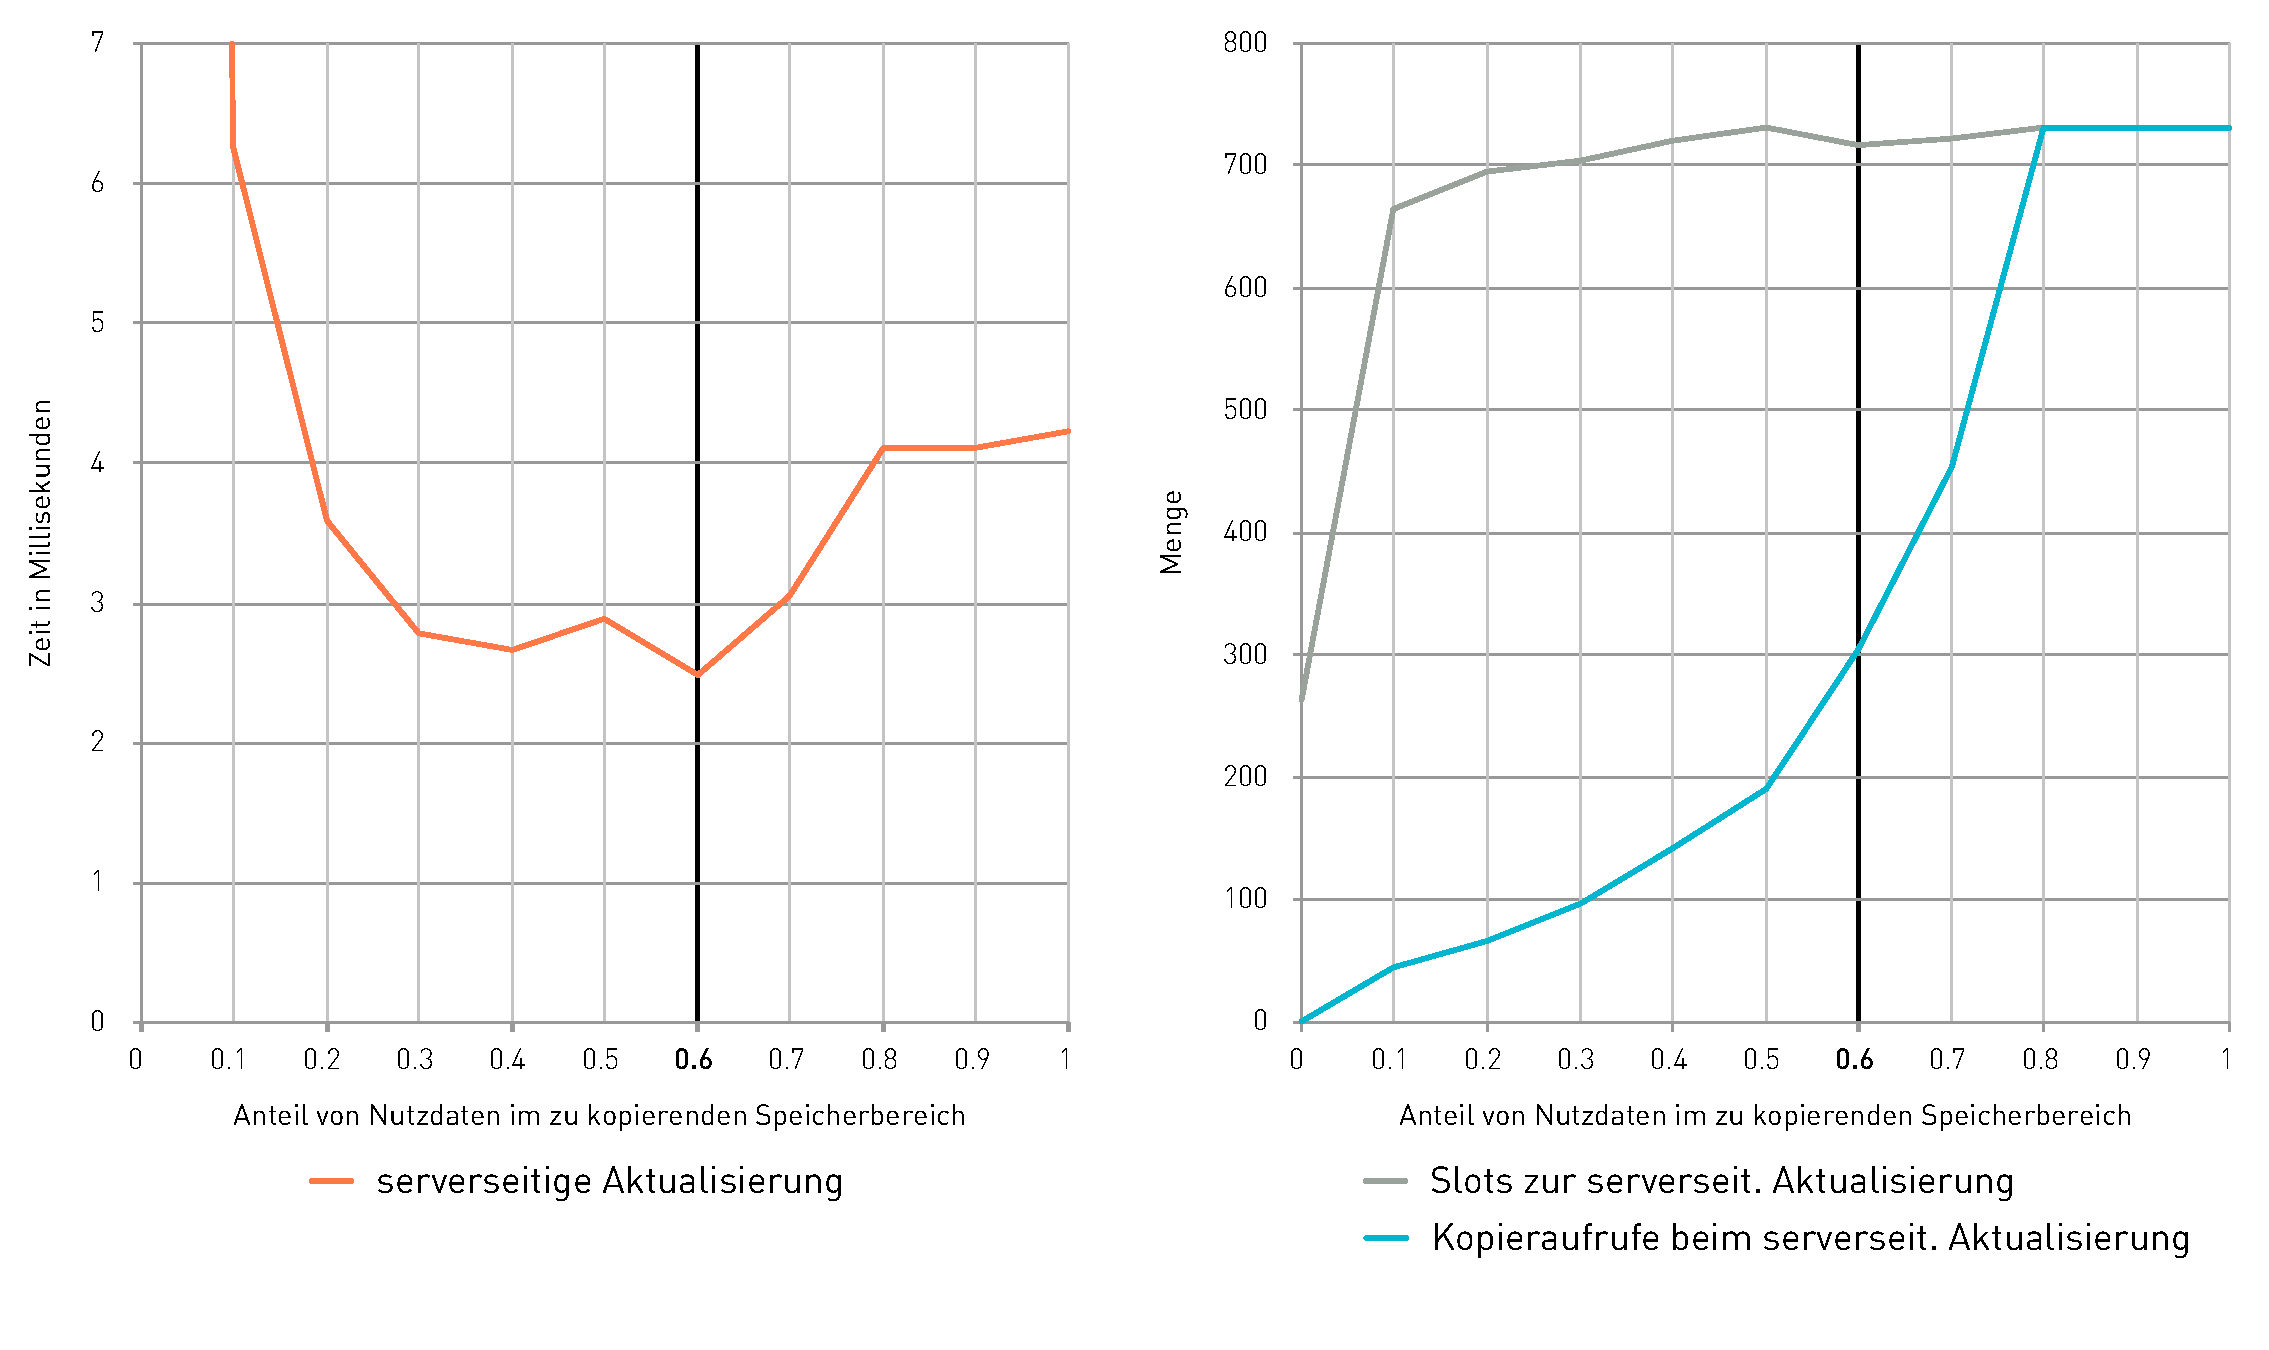
\includegraphics[width=1.0\textwidth]{figures/ratio_0-1.pdf}
  \caption{�fm�AFJa�FOJ\label{ratio_0-1}}
\end{figure}


\section{Einschr�nkungen und Verbesserungen}

\subsection{Serverseitige Aktualisierung}
Die in Abschnitt \ref{sec:serverseitige_aktualisierung} beschriebene Zusammenfassung der zu kopierenden Incore-Buffer-Slots wirkt sich deutlich auf die zum �bertragen der ge�nderten Speicherbereiche ben�tigte Zeit aus. Wie beschrieben arbeitet der Ansatz am besten wenn die zu transferierenden Speicherbereiche 
Mit steigender Fragmentierung des Incore-Buffers sinkt die Einsparung jedoch und schwankt stark. Bei einem vorgegebenen Verh�ltis zu aktualisierenden Slots von 20\% etwa schwankt die Einsparung zwischen 10\% bis 92\% und lag �ber einen Zeitraum von 60 Sekunden im Mittel bei etwa 43\%. Die hier examplarisch genannten Werte sind jedoch wenig aussagekr�ftig, da das Verhalten des Ansatzes nicht nur von der Anzahl der Slots, der Gr��e und dem Fragmentierungsgrad des Incore-Buffers abh�ngt, sondern auch von der Geometrie und der Kameraposition �ber die Zeit. Eine Verbesserung zum einzelnen Kopieren der Slots ist jedoch erkennbar.

\subsection{Verwendung von OpenGL Texturen als Buffer}
...
